%!TEX root = ../Thesis.tex
\chapter{Harmonic Oscillator - Hamilton's Equations and Numerical Analysis}

\section{Equations of Motion}
\begin{figure}[ht!]
\centering 
\includegraphics[scale=0.7]{fig/harmonic_oscillator.pdf}
\caption{The harmonic oscillator}
\label{fig:ho}
\end{figure}
\begin{description}
\item[Step 0 \quad Lagrangian $L$] \ \\[0.5cm]
Generalized coordinate: $x$. \\[0.2cm]
$T = \frac{1}{2} m \dot{x}^2.$ \\[0.2cm]
$V = \frac{1}{2} k x^2$ \\[0.2cm]
$L(x, \dot{x}) = T - V = \frac{1}{2} m \dot{x}^2 - \frac{1}{2} k x^2$

\item[Step 1 \quad Generalized momentum $p$] \ \\[0.2cm]
$p(x,\dot{x}) = \dfrac{\partial L}{\partial \dot{x}} = k \dot{x}$

\item[Step 2 \quad Transform $\dot{x}$] \ \\[0.5cm]
$\dot{x} = \dot{x}(x, p) = \dfrac{p}{k}$

\item[Step 3 \quad The Hamiltonian $H(\vec{q}, \vec{p}, t) = \sum\limits_{i=1}^n p_i \dot{q_i} - L$] \ \\
\begin{align}
\nonumber H &= p \cdot \dot{x} - \left(\frac{1}{2} m \dot{x}^2 - \frac{1}{2} k x^2\right) \\
\nonumber  &= p \cdot \dfrac{p}{m} - \left(\frac{1}{2} m \left(\frac{p}{m}\right)^2 - \frac{1}{2} k x^2\right) \\
&= \dfrac{p^2}{2m} + \dfrac{1}{2}k x^2
\end{align}
, which we recognize simply as the total energy. The first term is the kinetic energy in terms of the momentum $p$ and the second term is the potential energy $V$.

\item[Step 4 \quad Hamilton's Equations of Motion]
\begin{align}
\begin{split}
\label{eq:ho-eom}
\dot{x} = +\dfrac{\partial H}{\partial p} &= \dfrac{p}{m} ,
\\[0.2cm]
\dot{p}_x = -\dfrac{\partial H}{\partial x} &= - k x
\end{split}
\end{align}
\end{description}

\section{Numerical Analysis}
We will now solve the harmonic oscillator's equations of motion, \eqref{eq:ho-eom}. For simplicity we'll set $k = m = 1$. Note that by choice of $m=1$ the momentum $p$ is equal to the velocity $v$. The first step is to discretize the equations
\begin{alignat}{2}
&\dod{x}{t} = p  & \qquad \implies \qquad &\Delta x = p \Delta t \\[0.5cm]
&\dod{p}{t} = - x & \qquad \implies \qquad &\Delta p = - x \Delta t
\end{alignat}
The solution for this linear system of equations is well known and can be expressed as
\begin{align}
\begin{split}
\label{eq:ho-analytical}
x(t) = A \cos{\omega t} + B \sin{\omega t} \\
p(t) = -A \sin{\omega t} + B \cos{\omega t}
\end{split}
\end{align}
A good way to test the validity and precision a numerical method is to compare it's solution to a problem of which we know an analytical solution. Hence we will use the analytical solution \eqref{eq:ho-analytical} to analyze the $x(t)$ and $p(t)$ errors of the solutions found with the following three algorithms.

\subsection{Explicit Euler algorithm}
\begin{align}
\begin{split}
\label{al:ho-euler_e}
x_{i+1} &= p_i\Delta t + x_i \\
p_{i+1} &= -x_i\Delta t + p_i
\end{split}
\end{align}
In the explicit Euler, time step $i+1$ only reference values from the old time step $i$.

\subsection{Implicit Euler algorithm}
\begin{align}
\begin{split}
x_{i+1} &= p_{i+1}\Delta t + x_i \\
p_{i+1} &= -x_{i+1}\Delta t + p_i
\end{split}
\end{align}
In the implicit Euler, time step $i+1$ only reference the new values from the same time step. In general this leads to a system of equations that may not have an analytical solutions, and function roots would have to be found numerically using e.g. Newton Raphson. In the case of the harmonic oscillator we have a system of linear equations that can be solved analytically for $(x_{i+1},p_{i+1}$
\begin{align}
\nonumber &x_{i+1} = p_{i+1}\Delta t + x_i \\
\nonumber &p_{i+1} = -x_{i+1}\Delta t + p_i \\[0.4cm]
\nonumber & \Downarrow \\[0.4cm]
\nonumber &x_{i+1} - p_{i+1}\Delta t = x_i \\
\nonumber &p_{i+1} + x_{i+1}\Delta t = p_i \\[0.4cm]
\nonumber &\Downarrow \\[0.4cm]
\nonumber &\begin{bmatrix}
  1 & -\Delta t \\
  \Delta t & 1
\end{bmatrix}
\begin{bmatrix}
  x_{i+1} \\
  p_{i+1}
\end{bmatrix}
= \begin{bmatrix}
  x_i \\
  p_i
\end{bmatrix} \\[0.4cm]
\nonumber &\Downarrow \\[0.4cm]
&\begin{bmatrix} \label{al:ho-euler_i}
  x_{i+1} \\
  y_{i+1}
\end{bmatrix}
= \dfrac{1}{{\Delta t}^2 + 1}
\begin{bmatrix}
  1 & \Delta t \\
  -\Delta t & 1
\end{bmatrix}
\begin{bmatrix}
  x_i \\
  y_i
\end{bmatrix}
\end{align}

\subsection{Symplectic Euler algorithm}
\begin{align}
\begin{split}
\label{al:ho-euler_s1}
x_{i+1} &= p_{i+1}\Delta t + x_i  \\
p_{i+1} &= -x_i\Delta t + p_i
\end{split}
\end{align}
or
\begin{align}
\begin{split}
\label{al:ho-euler_s2}
x_{i+1} &= p_{i}\Delta t + x_i  \\
p_{i+1} &= -x_{i+1}\Delta t + p_i
\end{split}
\end{align}
In the symplectic Euler, time step $i+1$ reference the new values one the coordinate equation and the old $i$ value in the momentum equation. This mixing of time step values makes the Euler method symplectic, i.e. energy conserving.

In the first version \eqref{al:ho-euler_s1}, clearly $p_{i+1}$ needs to be run before $x_{i+1}$ in each time step. We can also do it the other way around as in \eqref{al:ho-euler_s2}. They give essential identical solutions. In this case the only difference is a phase shift of the momentum error by $\pi$ (Appendix \ref{app:symplectic_difference}).

Algorithms \crefrange{al:ho-euler_e}{al:ho-euler_s1} was implemented in Python (Appendix \ref{app:ho}).

\section{Plots}
\begin{figure}
    \centering
        \subbottom[Explicit Euler]{
            \includegraphics[scale=0.24]{fig/ho/ho_x(t)_euler_explicit.pdf}
            \label{fig:ho_x(t)_euler_explicit}
        }
        \subbottom[Implicit Euler]{
            \includegraphics[scale=0.24]{fig/ho/ho_x(t)_euler_implicit.pdf}
            \label{fig:ho_x(t)_euler_implicit}
        }
        \subbottom[Symplectic Euler]{
            \includegraphics[scale=0.24]{fig/ho/ho_x(t)_euler_symplectic.pdf}
            \label{fig:ho_x(t)_euler_symplectic}
        }
        \caption{Position x(t)}
    \label{fig:ho_x(t)_euler}
\end{figure}

\begin{figure}
    \centering
        \subbottom[Explicit Euler]{
            \includegraphics[scale=0.24]{fig/ho/ho_p(t)_euler_explicit.pdf}
            \label{fig:ho_p(t)_euler_explicit}
        }
        \subbottom[Implicit Euler]{
            \includegraphics[scale=0.24]{fig/ho/ho_p(t)_euler_implicit.pdf}
            \label{fig:ho_p(t)_euler_implicit}
        }
        \subbottom[Symplectic Euler]{
            \includegraphics[scale=0.24]{fig/ho/ho_p(t)_euler_symplectic.pdf}
            \label{fig:ho_p(t)_euler_symplectic}
        }
        \caption{Momentum p(t), equivalent to v(t) by choice of $m=1$}
    \label{fig:ho_p(t)_euler}
\end{figure}

\begin{figure}
    \centering
        \subbottom[Explicit Euler]{
            \includegraphics[scale=0.24]{fig/ho/ho_x(t)-error_euler_explicit.pdf}
            \label{fig:ho_x(t)-error_euler_explicit}
        }
        \subbottom[Implicit Euler]{
            \includegraphics[scale=0.24]{fig/ho/ho_x(t)-error_euler_implicit.pdf}
            \label{fig:ho_x(t)-error_euler_implicit}
        }
        \subbottom[Symplectic Euler]{
            \includegraphics[scale=0.24]{fig/ho/ho_x(t)-error_euler_symplectic.pdf}
            \label{fig:ho_x(t)-error_euler_symplectic}
        }
        \caption{Position x(t) error. Note the y-scale difference in symplectic \ref{fig:ho_x(t)-error_euler_symplectic}}
    \label{fig:ho_x(t)-error_euler}
\end{figure}

\begin{figure}
    \centering
        \subbottom[Explicit Euler]{
            \includegraphics[scale=0.24]{fig/ho/ho_p(t)-error_euler_explicit.pdf}
            \label{fig:ho_p(t)-error_euler_explicit}
        }
        \subbottom[Implicit Euler]{
            \includegraphics[scale=0.24]{fig/ho/ho_p(t)-error_euler_implicit.pdf}
            \label{fig:ho_p(t)-error_euler_implicit}
        }
        \subbottom[Symplectic Euler]{
            \includegraphics[scale=0.24]{fig/ho/ho_p(t)-error_euler_symplectic.pdf}
            \label{fig:ho_p(t)-error_euler_symplectic}
        }
        \caption{Momentum p(t) error}
    \label{fig:ho_p(t)-error_euler}
\end{figure}

\begin{figure}
    \centering
        \subbottom[Explicit Euler]{
            \includegraphics[scale=0.24]{fig/ho/ho_E(t)_euler_explicit.pdf}
            \label{fig:ho_E(t)_euler_explicit}
        }
        \subbottom[Implicit Euler]{
            \includegraphics[scale=0.24]{fig/ho/ho_E(t)_euler_implicit.pdf}
            \label{fig:ho_E(t)_euler_implicit}
        }
        \subbottom[Symplectic Euler]{
            \includegraphics[scale=0.24]{fig/ho/ho_E(t)_euler_symplectic.pdf}
            \label{fig:ho_E(t)_euler_symplectic}
        }
        \caption{Normalized energy E(t)}
    \label{fig:ho_E(t)_euler}
\end{figure}

\begin{figure}
    \centering
        \subbottom[Explicit Euler]{
            \includegraphics[scale=0.24]{fig/ho/ho_phase-space_euler_explicit.pdf}
            \label{fig:ho_phase-space_euler_explicit}
        }
        \subbottom[Implicit Euler]{
            \includegraphics[scale=0.24]{fig/ho/ho_phase-space_euler_implicit.pdf}
            \label{fig:ho_phase-space_euler_implicit}
        }
        \subbottom[Symplectic Euler]{
            \includegraphics[scale=0.24]{fig/ho/ho_phase-space_euler_symplectic.pdf}
            \label{fig:ho_phase-space_euler_symplectic}
        }
        \caption{Phase-space}
    \label{fig:ho_phase-space_euler}
\end{figure}

Things to note about the integrators from the figures \crefrange{fig:ho_x(t)_euler}{fig:ho_phase-space_euler}:
\begin{itemize}
    \item Explicit and implicit drift in position amplitude but stay true in phase.
    \item Symplectic drift in phase but stay true in amplitude (and thereby energy).
    \item In terms of energy, symplectic stays close to the analytic solution for much longer time. This is what defines a symplectic integrator and it is it's primary benefit.
    \item Explicit tends to add energy to the system (spiral outwards in phase-space plot), implicit ends to remove energy from the system (spiral inward in phase-space plot). Symplectic stays in the same orbit in phase-space, i.e. conserves the energy.
\end{itemize}

\subsection{The Two Symplectic Euler Methods Compared} \label{app:symplectic_difference}
We call the first version \eqref{al:ho-euler_s1} ``Symplectic1'' and the second version \eqref{al:ho-euler_s2} ``Symplectic2''. We see that they yield essential identical solutions. In this case the only difference is a phase shift of the momentum error by $\pi$ in figure \ref{fig:symplectic-difference}.
\begin{figure}
    \centering
        \subbottom[Symplectic1]{
            \includegraphics[scale=0.35]{fig/ho/ho_x(t)_euler_symplectic.pdf}
        }
        \subbottom[Symplectic2]{
            \includegraphics[scale=0.35]{fig/ho/ho_x(t)_euler_symplectic2.pdf}
        }
        \caption{Position x(t)}
\end{figure}

\begin{figure}
    \centering
        \subbottom[Symplectic1]{
            \includegraphics[scale=0.35]{fig/ho/ho_x(t)-error_euler_symplectic.pdf}
        }
        \subbottom[Symplectic2]{
            \includegraphics[scale=0.35]{fig/ho/ho_x(t)-error_euler_symplectic2.pdf}
        }
        \caption{Position x(t) error}
\end{figure}

\begin{figure}
    \centering
        \subbottom[Symplectic1]{
            \includegraphics[scale=0.35]{fig/ho/ho_p(t)_euler_symplectic.pdf}
        }
        \subbottom[Symplectic2]{
            \includegraphics[scale=0.35]{fig/ho/ho_p(t)_euler_symplectic2.pdf}
        }
        \caption{Momentum p(t)}
\end{figure}

\begin{figure}
    \centering
        \subbottom[Symplectic1]{
            \includegraphics[scale=0.35]{fig/ho/ho_p(t)-error_euler_symplectic.pdf}
        }
        \subbottom[Symplectic2]{
            \includegraphics[scale=0.35]{fig/ho/ho_p(t)-error_euler_symplectic2.pdf}
        }
        \caption{Momentum p(t) error. Note the difference in phase.}
    \label{fig:symplectic-difference}
\end{figure}

\begin{figure}
    \centering
        \subbottom[Symplectic1]{
            \includegraphics[scale=0.35]{fig/ho/ho_E(t)_euler_symplectic.pdf}
        }
        \subbottom[Symplectic2]{
            \includegraphics[scale=0.35]{fig/ho/ho_E(t)_euler_symplectic2.pdf}
        }
        \caption{Energy E(t)}
\end{figure}

\begin{figure}
    \centering
        \subbottom[Symplectic1]{
            \includegraphics[scale=0.35]{fig/ho/ho_phase-space_euler_symplectic.pdf}
        }
        \subbottom[Symplectic2]{
            \includegraphics[scale=0.35]{fig/ho/ho_phase-space_euler_symplectic2.pdf}
        }
        \caption{Phase-space}
\end{figure}